\chapter{Foreword}
\pg
write introduction to the thesis

\chapter{Introduction}
\minitoc

\pg
In this section, we contextualise the work done as part of this PhD by discussing the difficulties introduced by the combination of sparse $uv$-coverage and weak \emph{a priori} constraints on the sky brightness distribution. The conceptual framework we will rely on throughout this manuscript, the Radio Interferometer's Measurement Equation, is described in greater details in  \cref{section.RIME}. We will begin by discussing radio interferometry itself. We will then discuss the so-called \emph{imaging problem}, and end by discussing the \emph{calibration problem}. While in practice calibration is done before imaging, it is conceptually helpful to begin with imaging. Until we reach our introduction to radio interferometric calibration, we will therefore assume that calibration has been successfully carried out, and that we are working on the \emph{corrected visibilities}, i.e. gain-corrected visibilities. 

\pg
We start by linking interferometry to more concrete concepts: specifically, we will give a (very!) brief introduction to radio antennas and their characteristics. We will then use this introduction to contextualise the advantages and drawbacks of radio interferometry, along with the concrete technical problems that the method introduces.

% will make the ideas and basis of radio interferometry more accessible by allowing us to explain the abstractions that interferometry relies on in terms of simpler instrumental configurations. We will then introduce the concrete problems that interferometry introduces: both a recapitulation of the venerable Zernike-van Cittert theorem \citep[cf.][]{1934Phy.....1..201V} and the problem of incomplete $uv$-coverage.

\clearpage
% !TeX spellcheck = en_UK

\section{Overview of Radio Interferometric Techniques}\label{section.imaging}

\pg
In this section, we will cover the difficulties introduced by the combination of sparse $uv$-coverage and weak \emph{a priori} constraints on the sky brightness distribution. While we do not need to strictly base ourselves on the RIME formalism described in \cref{section.RIME}, it remains the conceptual framework we will assume that the reader uses. For the remainder of this section, we will assume that calibration has been successfully carried out, and that we are working on the \emph{corrected visibilities}, i.e. gain-corrected visibilities. 

\pg
We will begin by linking interferometry to more concrete concepts: specifically, we will give a (very!) brief introduction to radio antennas and their characteristics. This will make the ideas and basis of radio interferometry more accessible by allowing us to explain the abstractions that interferometry relies on in terms of simpler instrumental configurations. We will then introduce the concrete problems that interferometry introduces: both a recapitulation of the venerable Zernike-van Cittert theorem \citep[cf.][]{1934Phy.....1..201V} and the problem of incomplete $uv$-coverage.


%
%\pg
%There exists a wide variety of methods used in imaging, from the venerable CLEAN algorithm\footnote{For an excellent beginner's introduction to CLEAN, the author heartily recommends \url{https://www.cv.nrao.edu/~abridle/deconvol/node7.html}} to cutting-edge compressed sensing and subspace deconvolution methods. We will begin this section by introducing a mathematical framework in which the problem of deconvolution can be understood, and proceed, from there, to discuss some of the deconvolution algorithms which can be used.
%
%\pg
%The formalism used in this section is based, in part or in whole, on that used by Cyril Tasse in [DDF paper].

\section{A Brief Introduction to Radio Astronomy}

\pg
Radio astronomy consists of observing the electromagnetic field at very long wavelengths, which means using radio dishes. These dishes measure a voltage signal, proportional to variations in the electromagnetic field in the direction of sensitivity. Achieving good sensitivity with radio dishes means having a very large collecting area - in this respect, they behave exactly the same way as optical telescopes. Similarly, when well-designed, they are diffraction-limited - this means that, once again like optical telescopes, their resolution is limited by their diameter.

\pg
However, because radio frequencies are so much lower, achieving a resolution comparable to e.g. the HST requires extremely large dishes. While there exist telescopes, both old and new, which work on this principle (from Arecibo Observatory, shown in Fig. , to the upcoming FAST telescope in China, shown in Fig. )

\begin{figure}[h]
\centering
\begin{subfigure}{.43\textwidth}
\resizebox{\hsize}{!}{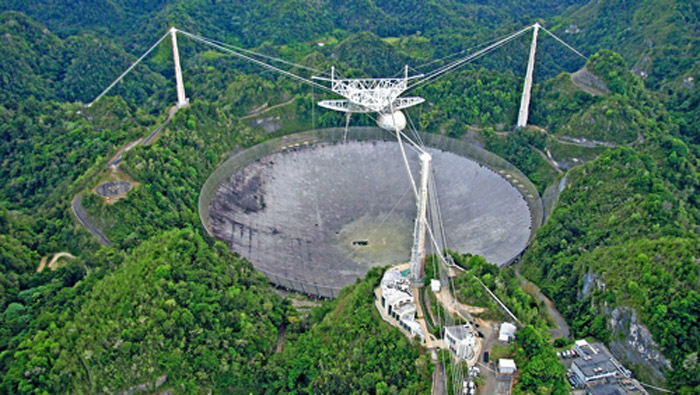
\includegraphics{images/20151101114231-0_8e7cc_c7a44aca_orig.jpg}}
\caption{\label{fig.arecibo} Arecibo telescope, in Puerto Rico.}
\end{subfigure}
\hfill
\begin{subfigure}{.43\textwidth}
\resizebox{\hsize}{!}{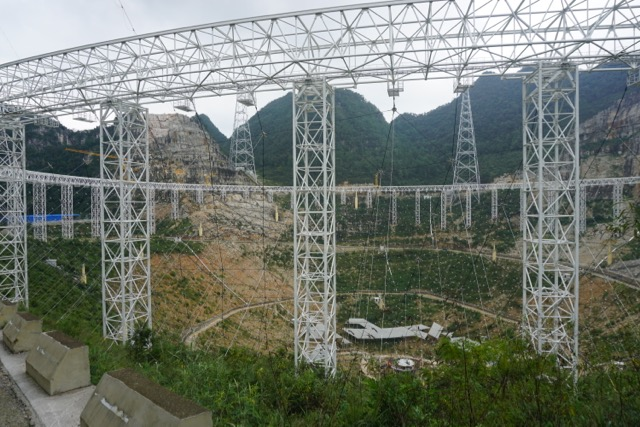
\includegraphics{images/FastTelescope_8sep2015.jpg}}
\caption{\label{fig.FAST} FAST telescope, in China}
\end{subfigure}
\caption{\label{fig.singleDishes} Examples of large single-dish radio telescopes.}
\end{figure}

\pg
Calibrating these dishes is a relatively straightforward matter - the signal loss and distortion as the dish converts the electromagnetic wave to a voltage can be described, based on the dish, either as a simple scaling factor, or a complex number (giving information on phase and amplitude errors). This loss and distortion model is referred to as the \emph{antenna gain}. Solving for these using more complex interferometric array is a problem described in Section \ref{section.calibration}.

\pg
For the remainder of this section, we will assume that calibration has been performed perfectly, and that the gain-corrections have been applied to voltage measurements. 

\section{Interferometry: Bypassing the Diffraction Limit}

\pg
There are two quantities of interest to astronomers of all stripes: sensitivity and resolution. An instrument's sensitivity is a function of its collecting area\footnote{It is also a function of technological factors, of course, but \emph{ceteris paribus}, a more sensitive telescope means a telescope with a wider collecting area}. Resolution, for well-designed instruments\footnote{By this, we mean that we assume that an instrument strives to optimise resolution.}, is limited by diffraction. This introduces issues specific to the radio domain. Radio waves, however, have very long wavelengths - often comparable to meters, rather than the 100$nm$ wavelengths of optical light. This introduces specific issues for astronomers, since achieving a resolution comparable to those of optical telescopes would require making telescopes with apertures tens of millions of times larger than those already titanic instruments!

\pg
To produce high-resolution maps of the radio sky, this technical limitation demands a technical solution. In practice, this solution consists of recourse to interferometric techniques. Indeed, interferometry can be thought of as the construction of a "sparse" dish, as illustrated in Fig.

\begin{figure}[h]
\centering
\begin{subfigure}{.43\textwidth}
\resizebox{\hsize}{!}{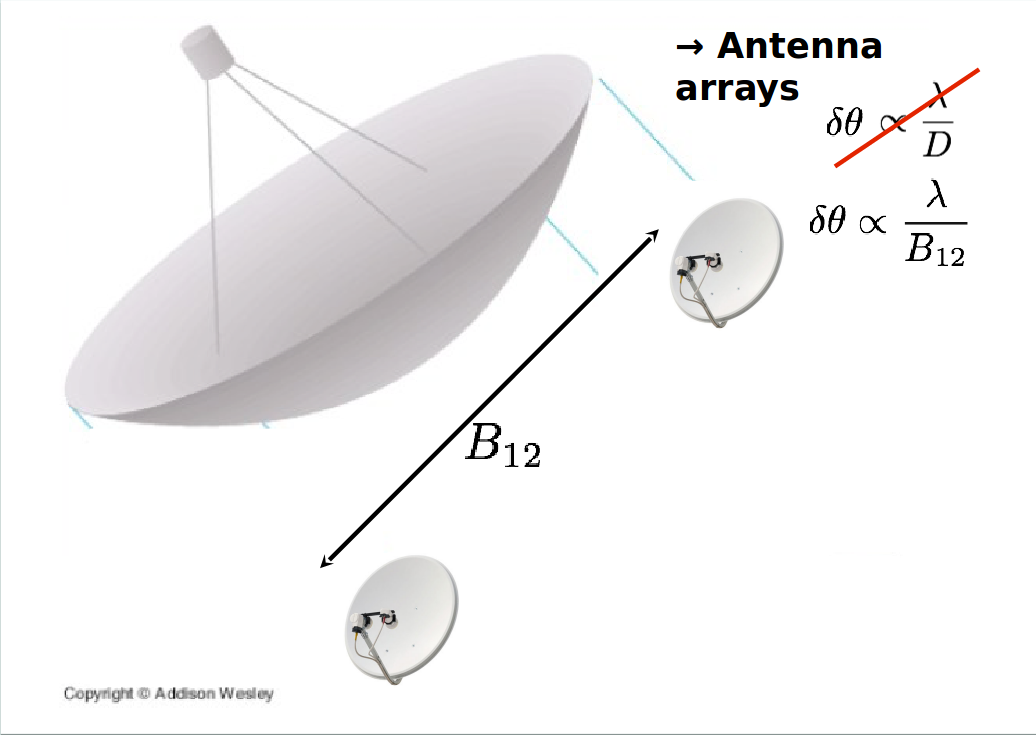
\includegraphics{images/baseline-resolution.png}}
\caption{\label{fig.baseline.image} A pair of dishes can surpass the resolution limit of its components.}
\end{subfigure}
\hfill
\begin{subfigure}{.43\textwidth}
\resizebox{\hsize}{!}{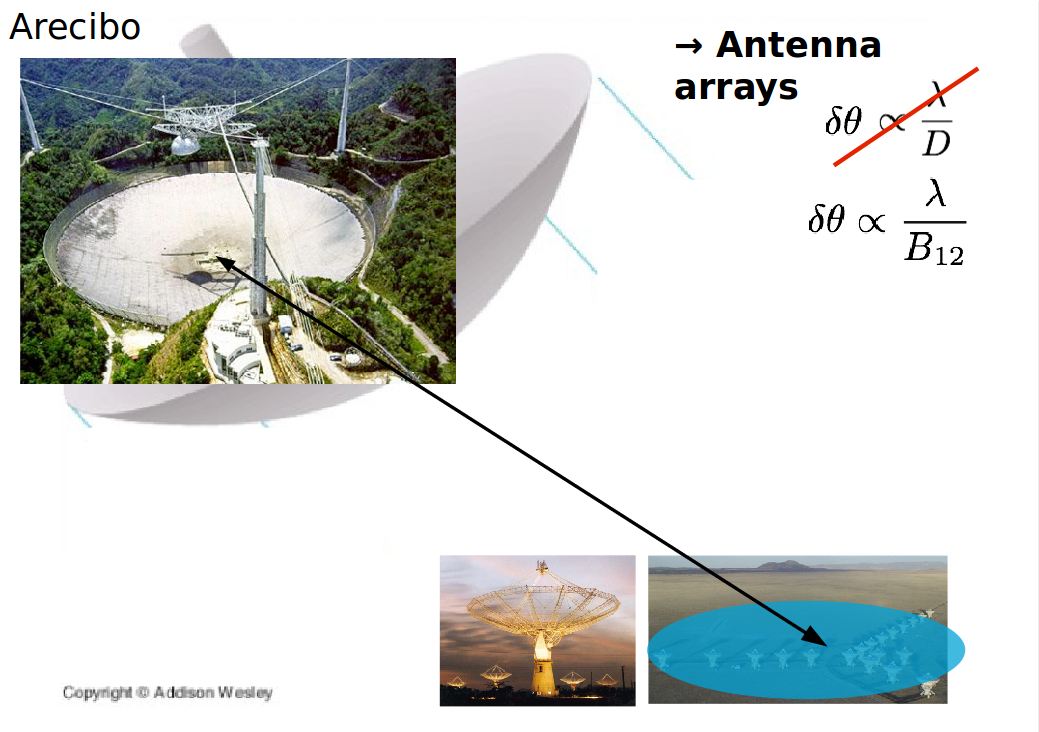
\includegraphics{images/arecibo-vla.png}}
\caption{\label{fig.arecibo.vla} With enough pairs of dishes, it is possible to synthesise a much larger dish.}
\end{subfigure}
\caption{\label{fig.aperture.synthesis} Illustration of the underlying principle of interferometry. The 27 dishes of the VLA can be thought of as "synthesising" a similar circular dish as Arecibo. This idea is the reason why radio interferometry is historically known as "aperture synthesis" in the literature of radio astronomy. Both images are copyrighted by Addison Wesley.}
\end{figure}

\pg
Of course, this improvement of resolution does not come for free. To understand the cost of interferometry, let us discuss the properties of its core component: the baseline.

\subsection{The Baseline}

\pg
To define the baseline, we must begin by considering the geometric properties of an interferometric array. For now, let us assume that we are observing the sky above the array, a practice known as drift-scanning. A baseline then consists of the vector subtraction of the positions, in 3-dimensional space, of its two constituent antennas. Note that each antenna pair therefore has 2 corresponding baselines, since for each pair of antennas A and B we have baselines AB and BA. These distance vectors are then divided by the observing wavelength to give a dimensionless set of coordinates, known as $(u,v,w)$. These coordinates define the baseline entirely. 

\subsection{The Visibility}

\pg
We have defined what a baseline corresponds to: a vector coordinate in $(u,v,w)$-space. To each baseline we associate a measurement, which we call the \emph{visibility}. 
\begin{figure}[h]
\centering
\resizebox{\hsize}{!}{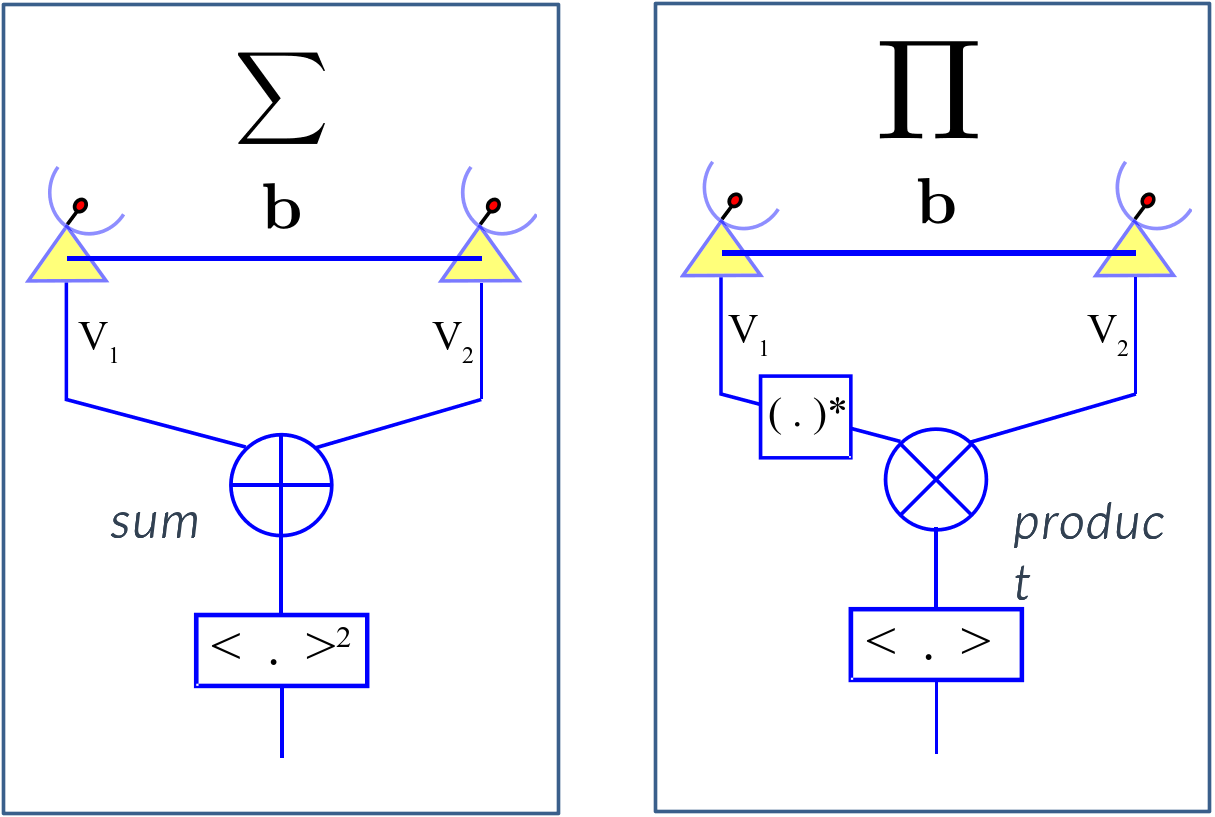
\includegraphics{images/visibility-creation.png}}
\caption{\label{fig.visibility} There are two ways to combine the voltages from two antennas into a visibility: they are sum-correlation and $\pi$-correlation. In this manuscript, we will only concern ourselves with the latter. Image credit: Julien Girard}
\end{figure}
The visibility associated with baseline $\mathbf{b}_{AB}$ is created by taking the voltage measured by antenna A, multiply it by the complex conjugate of the voltage measured by antenna B, average over the correlator dump time (i.e. the time over which the measurement is made). This scalar quantity is then multiplied by the baseline position vector. In other words:
\begin{equation}
\mathbf{b}_{AB} = V_{A} V_{B}^* \frac{\mathbf{x}_{B}-\mathbf{x}_{A}}{\nu_\mathrm{obs}}
\end{equation}

\pg
So we see that a visibility is a complex vector quantity. We also see that $\mathbf{b}_{AB} = \mathbf{b}_{BA}^*$: the information of the visibility associated with baseline BA is contained in the visibility associated with baseline AB. This means that in practice, only half of the visibilities ever need be stored. What does the visibility measurement correspond to?
\begin{figure}[h]
\centering
\resizebox{\hsize}{!}{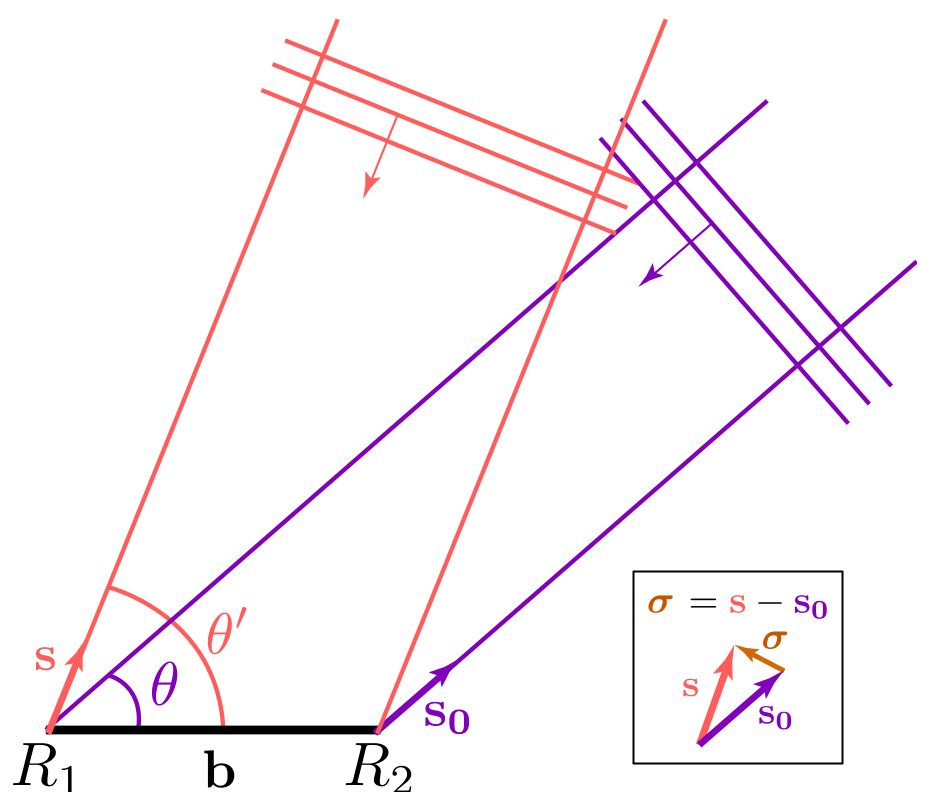
\includegraphics{images/visibility-measure.png}}
\caption{\label{fig.visibility.measure} Here, we assume that there are only two sources in the sky whose signal can be measured by our antennas. The final visibility is the sum of the visibilities associated with each individual source. Image credit: Julien Girard}
\end{figure}

\pg
The signals from various sources are additive in both antennas. Provided that the signal from both sources is coherent when observed by the dishes, the correlation between the total voltages will simply be the sum of the voltage correlations associated with individual sources - i.e. the interferometric signal from different sources are additive.

\pg
Note that in Fig. \ref{fig.visibility.measure}, neither source is at the zenith. We thus see that the \emph{effective baseline} which sees each source is in fact shorter than the \emph{physical baseline}. This can be corrected by digitally adding a phase delay in each antenna (or, in older interferometers, by playing with the cable length between each dish and the correlator) - this is in fact how interferometric arrays are pointed.

\subsection{The $uv$-plane}

\pg
In general, interferometric design is such that the $w$ component of visibilities' $(u,v,w)$ coordinates is negligible (or can be put in a frame of reference where it can usually be approximated as such). Radio astronomers tend to thus talk of a $uv$-plane rather than $uvw$-space to describe the space where visibilities live. The set of $uv$-values for all the baselines of an interferometric array is known as its $uv$-coverage, and defines the array's properties entirely.

\pg
For the VLA, for example, the $uv$-coverage when observing the zenith will be as shown in Fig. \ref{fig.vla.uvcoverage}.

\begin{figure}[h]
\centering
\resizebox{\hsize}{!}{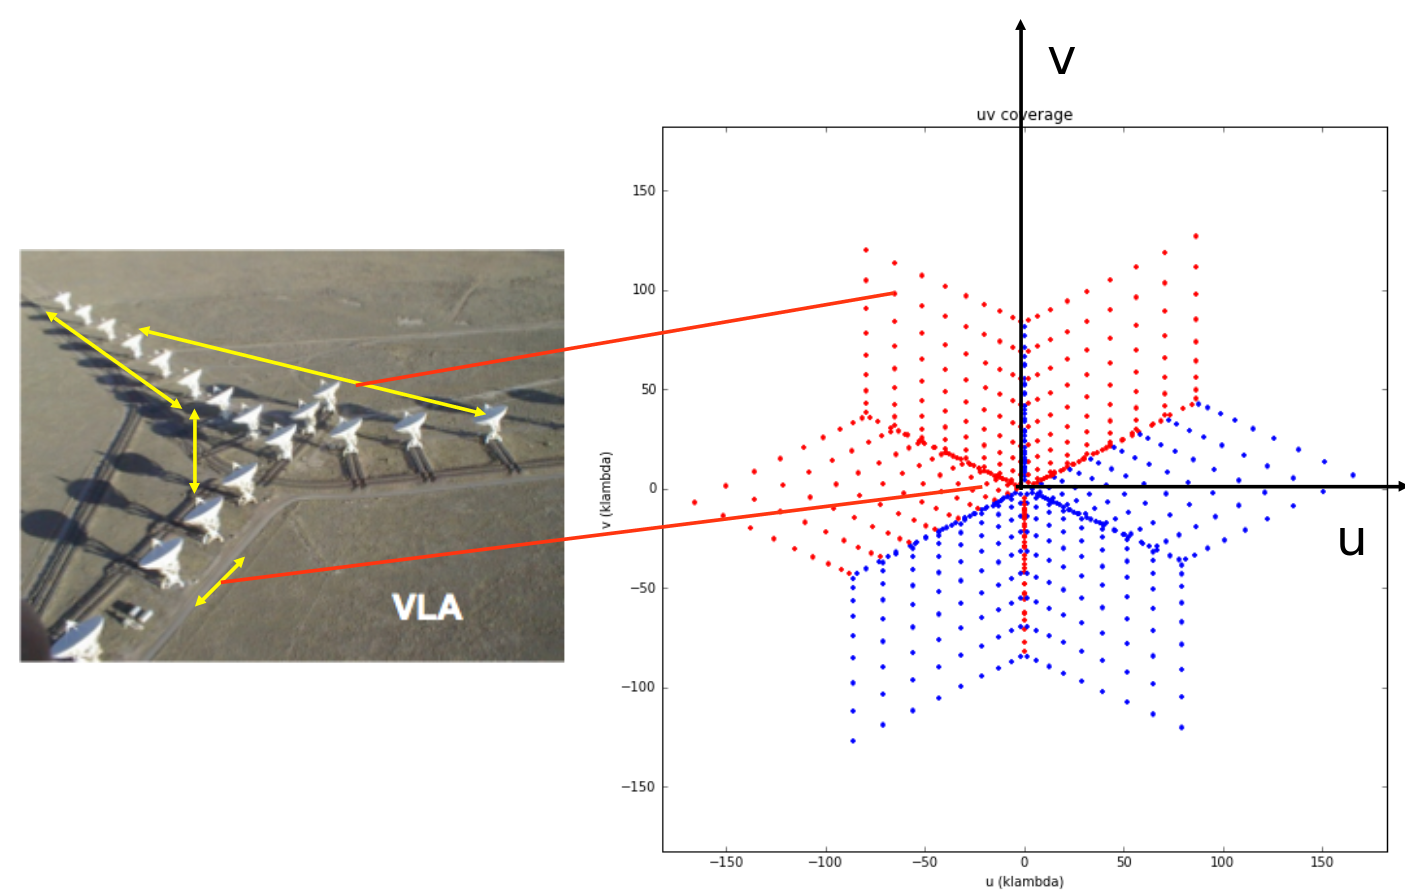
\includegraphics{images/vla-uvcoverage.png}}
\caption{\label{fig.vla.uvcoverage} The VLA contains 27 radio dishes placed as shown above. Each antenna pair between those 27 gives two single baselines, here, one red and one blue. Image credit: Julien Girard}
\end{figure}

%\pg
%The more points an array has in $uv$-space, the greater its $uv$-coverage and the better it will observe. This coverage can be improved for free in two main ways: firstly, the use of a technique known as supersynthesis (since the interferometer "synthesises" a dish at any given time, by assuming that the sky does not evolve over a certain time frame, we can treat different times as measurements of the same sky) and taking advantage of the frequency-dependence of $uv$-coordinates.The impact of both practices will be described in greater detail in \ref{sec.imag.psf}, but know that "$uv$-tracks" simply correspond to the $uv$-coverage of an interferometer observing over some period of time.

\pg
Individual antennas of an array can be pointed mechanically, and so the impact of pointing the interferometric array in a given direction can be minimised. But what happens to the array itself? It is useful here to go back to the illustration of Fig. \ref{fig.arecibo.vla}. Think of each dish in the array representing a "filled" segment of a massive but empty dish. By projecting our observation in a given direction, this dish goes from circular to elliptical.
\begin{figure}[h]
\centering
\begin{subfigure}{.40\textwidth}
\resizebox{\hsize}{!}{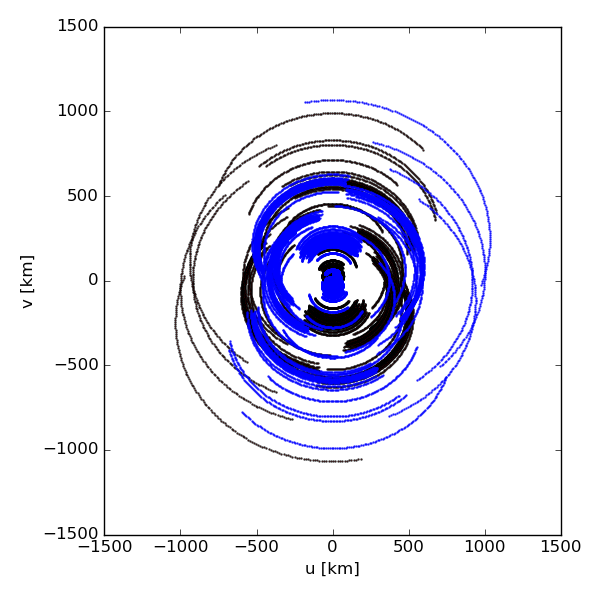
\includegraphics{images/lofar-uvcoverage-zenith.png}}
\caption{\label{fig.lofar.uvcoverage.zenith} $uv$-coverage of an 8-hour LOFAR observation when pointing at zenith..}
\end{subfigure}
\hfill
\begin{subfigure}{.40\textwidth}
\resizebox{\hsize}{!}{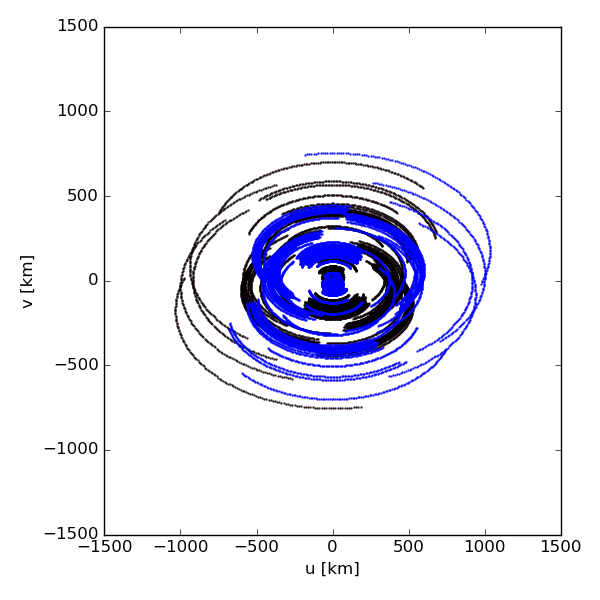
\includegraphics{images/lofar-uvcoverage-elsewhere.png}}
\caption{\label{fig.lofar.uvcoverage.elsewhere} $uv$-coverage of an 8-hour LOFAR observation when pointing 45 degrees away from zenith.}
\end{subfigure}
\caption{\label{fig.uvcoverage.lofar} Effect of array pointing on $uv$-coverage. By pointing the array 45 degrees in the $v$-axis, the array's $uv$-coverage (and thus maximum resolution) is decreased along the $v$-axis.}
\end{figure}


\subsection{The Point-Spread Function}\label{sec.imag.psf}

\pg
So far, we have seen that the purpose an interferometric array is to overcome the diffraction limit of single-dish antennas. We have described visibilities, which are the quantities measured by an interferometric array. What remains is to describe how these measurements are used to go make images of the sky.

\pg
Assuming that all the antennas in an array are equivalent and perfectly calibrated, the van Cittert-Zernike theorem (\citepads{1934Phy.....1..201V}, covered in \citepads{2001isra.book.....T}) allows us to equate a visibility with a single Fourier mode of the plane tangent to the sky where the instrument is pointed. This direction is called the \emph{phase centre}, because digital phase shifts are introduced between antenna voltages before averaging so as to point each visibility in this direction. 

\subsection{From Dirty to Clean: Mitigating the PSF}

\clearpage
% !TeX spellcheck = en_UK

\section{Calibration Methods in Radio Interferometry}\label{section.calibration}
\pg
In this section, we will discuss the implementation of interferometric array calibration. Our analysis is based on the RIME formalism, described in \cref{section.RIME}. One key metric of calibration quality is the \emph{dynamic range} (DR). High dynamic ranges mean that a high contrast has been obtained, and fainter sources can be reached. Dynamic range is defined as the following:
\begin{equation}\label{eq.DR}
DR = \frac{flux_{max}}{\max(\sigma_{thermal},\sigma_{artefacts})}
\end{equation}
where $flux_{max}$ is the flux of the brightest source, $\sigma_{thermal}$ the thermal noise in the image, and $\sigma_{artefacts}$ the noise associated with calibration artefacts.

\pg
The distinction between these two noise sources is crucial; one can never go `below noise' for a given observation, no matter the quality of calibration. Astronomers typically observe for longer periods of time in order to reduce $\sigma_{thermal}$ in their images, but this will not reduce the artefacts caused by poor calibration solutions. However, uncorrected Direction-Dependent Effects will not go away on their own, no matter how long the integration time.

\pg
There are three `generations' of calibration methods, of increasing complexity. I shall describe them in terms of the RIME, showing how each generation increases in generality to account for more exotic effects. For the sake of clarity, I shall henceforth refer to them interchangeably as `nth-generation calibration' or `nGC' methods.

\subsection{Generational Analysis}

\subsubsection{First-Generation: Open-Loop Calibration}\label{section.calibration.1gc}

\pg
First-generation calibration methods (1GC methods) consist of open-loop calibration. This relies entirely on instrument stability, and thus imposes significant design constraints on radio telescopes. It consists of briefly observing a calibrator before and after each observation run to find a gain factor and offset error\footnote{For a concrete example, see \href{http://www.analog.com/en/analog-dialogue/articles/open-loop-calibration-techniques.html}{here}.}

\pg
Phase calibration in the 1GC era `proper' was not done, as engineers were capable of ensuring phase stability in contemporary interferometers. Phase was thus calculated relative to a fixed frame of reference, usually the central antenna of a 3-antenna array. 

\pg
In RIME terms, this consists of solving for a very basic form of $\Gjones_p$:
\begin{equation}
\Gjones_p = \begin{bmatrix} a_p t + b_p \end{bmatrix} % \begin{bmatrix} e^{2 \pi i \nu ( \phi_p - \phi_0)} \end{bmatrix}
\end{equation}
where $a_p,b_p$ are constants solved for during open-loop calibration and $t$ is time. %, $\nu$ the observing frequency, $\phi$ the phase at an antenna, and $\phi_0$ the phase at the reference antenna.

\pg
While values for $a_p$ and $b_p$ can in theory be found for both autocorrelation and both crosscorrelations, low signal-to-noise means that in practice, a single set of values is solved for per antenna\footnote{This reduces calibration to solving only for the intensity gains: the data can then only be used for \emph{intensity mapping} (e.g. \citepads{1957IAUS....4..159J}). This practice therefore precludes polarimetry.}. With these techniques, one can achieve dynamic ranges of about 100:1 (\citepads{2010A&A...524A..61N}).

\subsubsection{Second-Generation: Self-Calibration}\label{section.calibration.2gc}

\pg
Second-generation calibration methods (2GC methods) are defined by their use of \emph{self-calibration}\footnote{On the discovery of self-calibration and its evolution in parallel to adaptive optics, I highly recommend the chapter titled "The Almost Serendipitous Discovery of Self-Calibration'' in "\href{http://library.nrao.edu/public/collection/02000000000280.pdf}{\citep{serendipitous}}.}, commonly referred to as \emph{self-cal} (\citepads{1984ARA&A..22...97P}). As described in \cref{section.RIME.FullSky.CVZ}, this method can only be deployed if the brightness matrix of the sky is the same for all baselines\footnote{This is not to say that the brightness matrix must contain only point sources, but rather that moving our interferometer 500m to the East should not change its measured visibilities} (i.e. that we are not affected by direction-dependent effects).

\pg
The seeds of self-calibration (and adaptive optics) is a paper published in the era of 1GC by Jennison (\citepads{1958MNRAS.118..276J}, expanding on his PhD work, which was published in 1951). With sufficient signal-to-noise, he showed that \emph{phase closure} could be calculated and errors due to the atmosphere thus mitigated.

\pg
Self-calibration and adaptive optics are the same thing, albeit meeting different constraints. Most notably, interferometric data is digital, allowing radio astronomers to perform their adaptive optics correction after the observation.

\pg
[ TODO: put adaptive optics diagram here maybe]

\pg
If amplitude and phase gains can be written as antenna-dependent, then each antenna-based error is estimated N times (once per baseline which includes this antenna). By estimating, and correcting for, these errors, one can use a simple source model to infer an improved one. This is why the method is referred to as self-cal; by calibrating `on' a good calibrator source (bright, compact and unresolved), one can drastically improve one's source model, along with one's calibration solutions.

\pg
By extending this idea to VLBI\footnote{e.g.  \citepads{1974ApJ...193..293R}}, \emph{amplitude closure} was introduced to the field along with phase closure \citepads[as described in][]{1983Sci...219...51R}. Astronomers were quick to apply these methods to interferometers in general.

\pg
The great advantage of radio interferometry over optics, however, is that we can \emph{iterate} over progressively improved source models. This is because interferometric data is digital, and because we record phase information.

\pg
In practice, of course, self-cal will be limited by noise. More precisely, it will be limited by sensitivity, in the form of the signal-to-noise ratio (henceforth SNR). For sufficiently bright sources, with high SNR, self-calibration can easily improve dynamic range by a factor of 10 (\cite{serendipitous}, p. 154) in a single iteration. 

\subsubsection{Third-Generation: Direction-Dependent Effects}

\pg
Third-generation calibration (3GC) is an extension of 2GC calibration which takes direction-dependent effects into account. At the time of writing, this is the cutting edge in radio interferometric calibration.

\pg
In this section, I will discuss the approach taken by [cite DDF and kMS paper when it comes out] and [cite prefactor paper if/when it is out], \emph{facet-based calibration}. This method has an imaging equivalent \citepads[see][and associated papers]{2017arXiv171202078T}. The approach cannot be divorced from imaging, for the simple reason that solving for and applying Jones matrices in different directions requires image-plane knowledge of the sky brightness distribution $\Bmatrix$. The imaging challenges this methods introduces will be discussed in [href to relevant imaging section].

\pg
The crucial insight of this approach consists 







\clearpage

\section{The Low-$\nu$ Sky: Emission Mechanisms}
\pg
This section aims to bring a brief introduction to the emission mechanisms which dominate at low frequencies, and thus determine the physics accessible to extragalactic astronomers working in this band. Specifically, it will briefly describe thermal radiation detected at low frequencies (associated with dust \& protoplanetary disks, and therefore a tracer of star formation) along with free-free radiation (which is emitted from ionised plasma outflows, and thus a tracer of various physical objects e.g. young stellar objects - cf. \citet{2017ApJ...834..206C} - and starburst regions - cf. \citet{2015A&A...574A.114V}) and synchrotron radiation, which is a tracer of more violent and energetic processes (and thus associated with supernova remnants, AGN, or radio halos - cf. \citet{2010A&A...509A..68C}).

\pg
Of course, each individual galaxy will have differing contributions from different mechanisms - in practice, when studying galactic populations, the overall flux at a given frequency will simply be summed up for each galaxy and become one point in a Spectral Energy Distribution, or SED. However, when studying individual objects, it can be critical to understand which emission mechanism dominates at what frequencies. %: it will be very difficult to find traces of star formation in the emission from a galaxy dominated by an AGN, for example. Along with a brief introduction of the main emission mechanisms, then, we will give the characteristic spectrum of each, to show how different types of emission can be differentiated in practice.
For example, the radio and far-infrared spectrum for nearby M82 are shown in Fig. \ref{plot.m82.spectrum}\footnote{Figure and work taken from the NRAO website. For further information, \href{https://www.cv.nrao.edu/course/astr534/FreeFreeEmission.html}{see here}}.
\begin{figure*}[!h]
\centering
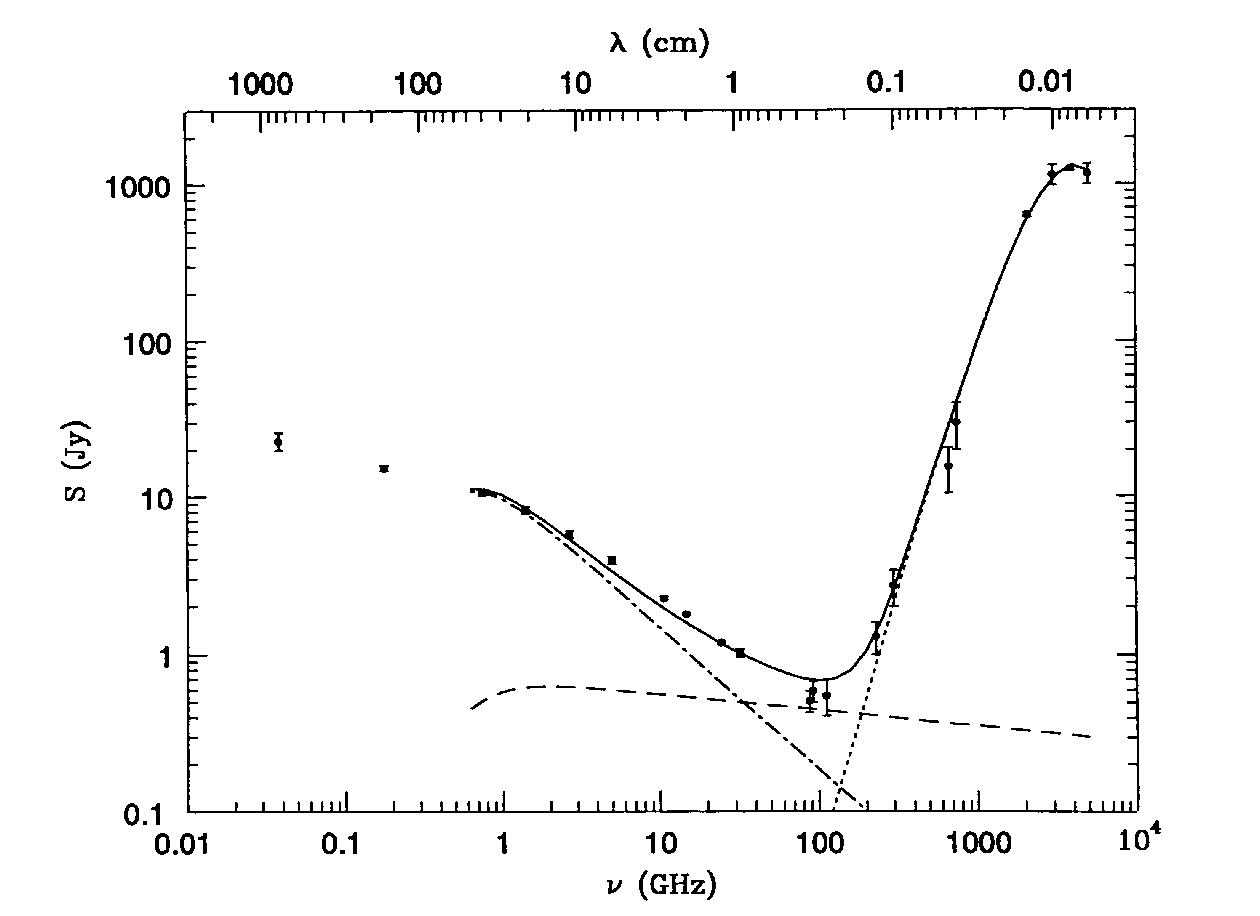
\includegraphics[width=\textwidth]{images/M82Spectrum.png}
\caption{\label{plot.m82.spectrum} Radio and far-infrared spectrum for galaxy M82, as estimated \href{https://www.cv.nrao.edu/course/astr534/FreeFreeEmission.html}{by the NRAO online course}. The flat curve corresponds to free-free emission, while synchrotron radiation and thermal dust emission dominate at low and high frequencies respectively.}
\end{figure*}

\pg


\subsection{Thermal Radiation}
\pg
Also known as black-body radiation, its spectral intensity is given by Planck's law, given in Eq. \ref{eq.planck}.
\begin{equation}\label{eq.planck}
%B_\lambda (\lambda,T) = \frac{2hc^2}{\lambda^5}\left(e^{\frac{hc}{\lambda k_BT}}-1\right)^{-1}
B_\nu(\nu,T) = \frac{2h\nu^3}{c^2}\left(e^\frac{h\nu}{k_BT}-1\right)^{-1}
\end{equation}
where $B_\lambda$ is the flux density at frequency $\nu$ for a source with temperature $T$, and $k_B=1.381 \left[J/K\right]$ is the Boltzmann constant. Near protostellar disks, synchrotron emission is absorbed by the ambient interstellar medium, heating it up to an average of $\sim 10^4$ (see \citetads{2009ApJS..181..255A}, \citetads{1978ppim.book.....S} and references therein). This gives the following spectral curve:

\begin{figure*}[!h]
\centering
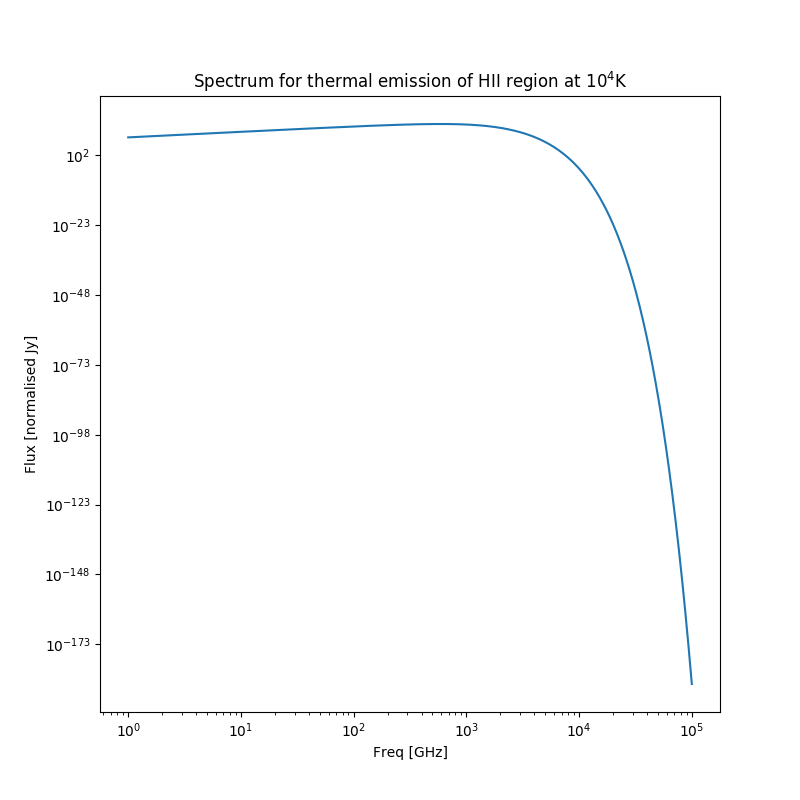
\includegraphics[width=0.8\textwidth]{images/ThermalEmission.png}
\caption{\label{plot.thermal}Log-Log plot of blackbody radiation emitted by a particle at $10^4$ Kelvin. Note that the y-axis is arbitrary, since it will in practice be modulated by the number of particles in a region, radiation efficiency, resolution etc.}
\end{figure*}
\pg
This is the dominant mode of emission for distant galaxies in the infrared band. In the LOFAR regime, it is not expected to dominate for extragalactic sources, but ought to be detected for resolved galaxies.

\subsection{Free-Free Radiation}
\pg
Free-free or ``bremsstrahlung" (``braking") radiation occurs when the trajectory of a high-energy charged particle is deflected by an electric field. This non-thermal emission mechanism is the dominant mechanism in HII regions (which contain ionised hydrogen), where star formation has previously taken place. It is called free-free emission because it is produced by free electrons scattering off ionised hydrogen without being captured. % as shown in Fig. \ref{plot.freefree}
%\begin{figure*}[!h]
%\centering
%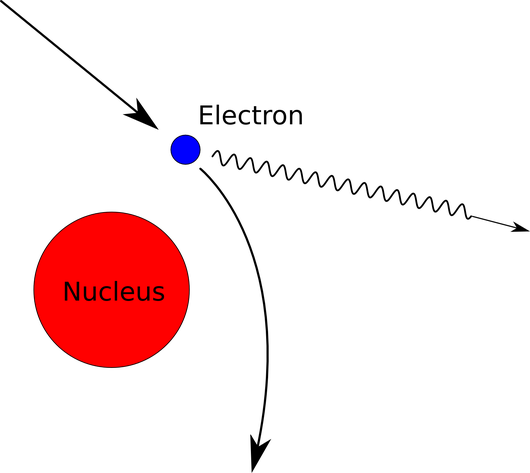
\includegraphics[width=0.3\textwidth]{images/bremsstrahlung.png}
%\caption{\label{plot.freefree} Schematic showing the physical process leading to free-free emission. As we can see, the electron is scattered, but not captured. Source: \url{https://thephysicsbehind.com/2015/04/16/x-ray-tubes/}}
%\end{figure*}

\pg
This emission's spectrum is heavily dependent on a number of factors: including frequency, temperature, and critically, free-free opacity $\tau_\nu$, itself a function of electron density. It is characterised by a knee in its spectrum, occurring where $\tau_\nu\sim 1$. This knee delineates two regions with different spectral indices; $\alpha \sim -0.1$ at higher frequencies, and $\alpha \leq 2$ at lower frequencies. This gives a characteristic shape, shown in Fig. \ref{plot.freefree.spectrum}.
\begin{figure*}[!h]
\centering
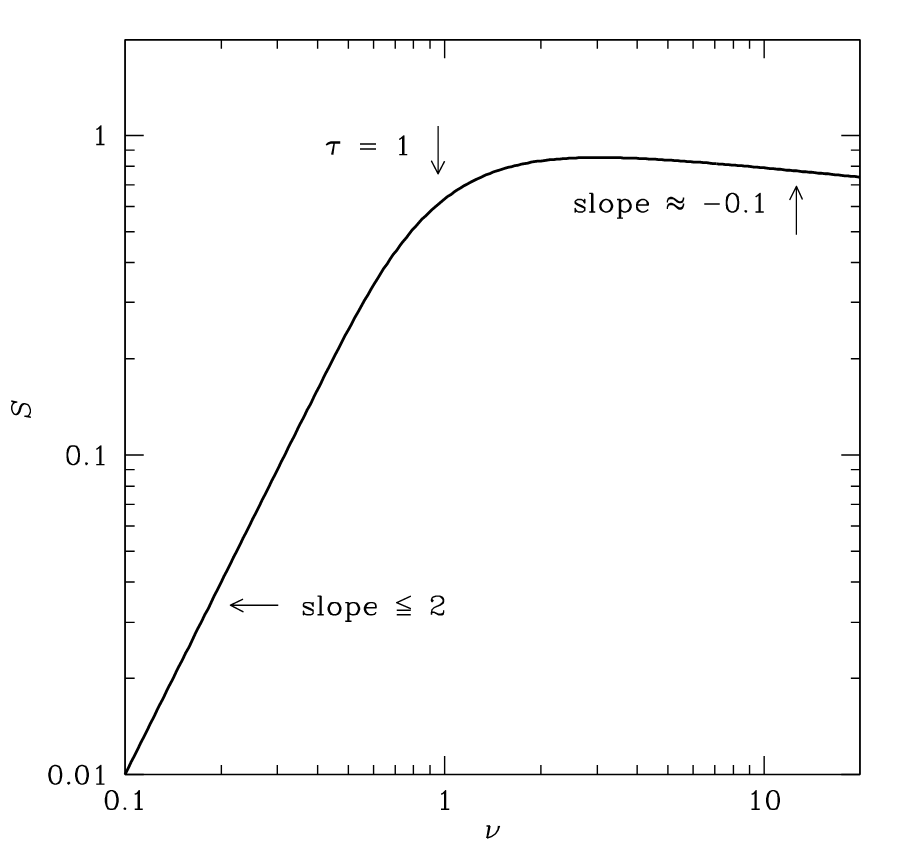
\includegraphics[width=0.9\textwidth]{images/freefree.png}
\caption{\label{plot.freefree.spectrum} Characteristic spectrum of free-free radiation. Arbitrary unit scale. Source: NRAO online course.}
\end{figure*}

\pg
As we can see, this spectrum falls off sharply with frequency. As such, while it is expected to dominate over thermal emission in the absence of synchrotron radiation, it is unlikely to dominate in the LOFAR band. It acts as a tracer for star formation and other "gentler" physical processes detected at low radio frequencies.

\subsection{Synchrotron Radiation}
\pg
Synchrotron radiation (or "magnetobremsstrahlung") occurs when the trajectory of a high-energy charged particle is deflected by a magnetic field. As the German name suggests, it is the magnetic equivalent of free-free radiation. It is the tracer of extremely violent processes, such as AGN jets. In its mildly relativistic regime, it is referred to as cyclotron radiation, after the device in which it was first tested, and in non-relativistic regimes, it is known as gyro radiation. 

\pg






\clearpage
\section{LOFAR: The LOw-Frequency Array}

\pg
In this section, we will describe the LOw Frequency Array LOFAR \citepads{2013A&A...556A...2V}, its technical properties and its current state of the art. In particular, the distinction between "Dutch" LOFAR and "international" LOFAR - and the technical problems associated with each - will be made explicit in this section.

\pg
LOFAR is a SKA pathfinder instrument, which means that it serves not only as a cutting-edge instrument in its own right, but does so with the explicit aim of serving as testing grounds for technologies \& techniques which could be usefully implemented in the SKA. It is in this context, for example, that trailblazers such as NeNuFar \citepads{2012sf2a.conf..687Z}, a low-frequency extension of LOFAR, are tested. LOFAR is an interferometric array, meaning that it consists of antennas which are combined to form stations, which are themselves distributed throughout the Netherlands and Europe.
\begin{figure}[h!] 
  \begin{minipage}[c]{0.45\linewidth}
    \centering
    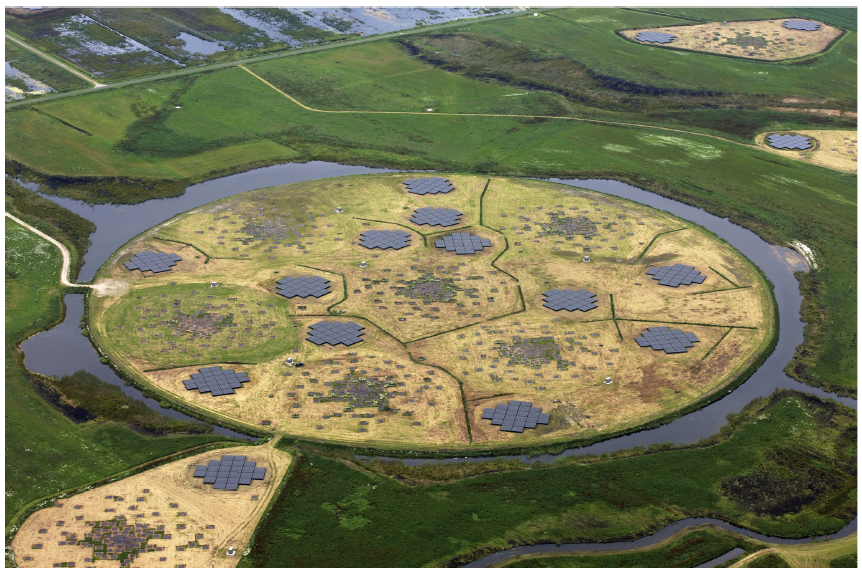
\includegraphics[width=\linewidth]{images/superterp.png}
	\subcaption{\label{fig.lofar.superterp} LOFAR core, known as the Superterp.}
%    \vspace{4ex}
  \end{minipage}
  \hfill
  \begin{minipage}[c]{0.45\linewidth}
    \centering
    \includegraphics[width=.5\linewidth]{images/{lofar-core-map_grey.jpg}}
    \subcaption{\label{fig.lofar.core} Distribution of the so-called LOFAR "core" stations, which include the Superterp.}
%    \vspace{4ex}
  \end{minipage} 
  \begin{minipage}[c]{0.45\linewidth}
    \centering
    \includegraphics[width=\linewidth]{images/{Distribution_Remote_Stations}} 
    \subcaption{\label{fig.lofar.remote} LOFAR with both "core" and "remote" stations.}
%    \vspace{4ex}
  \end{minipage}
  \begin{minipage}[c]{0.45\linewidth}
    \centering
    \includegraphics[width=.9\linewidth]{images/{Distribution_International_Stations}} 
    \subcaption{\label{fig.lofar.international} International LOFAR. Newer stations (one in Ireland, three in Poland) are not shown here.}
%    \vspace{4ex}
  \end{minipage} 
\caption{\label{fig.lofar.distribution} Geographic location and distribution of LOFAR stations, explicitly showing what is meant by Superterp, core, remote and international stations. All images from \href{https://www.astron.nl/radio-observatory/astronomers/users/technical-information/lofar-array-configuration/lofar-array-conf}{the official ASTRON website}}
\end{figure}


\pg
There are two bands to LOFAR, which are known as LOFAR-HBA (High-Band Antennas) and LOFAR LBA (Low-Band Antennas). \cref{fig.lofar.superterp,fig.fr606.layout} show the layout of the 6 innermost core stations and the French international LOFAR station, respectively.
\begin{figure}[h!]
\includegraphics[width=0.5\textwidth]{images/{LOFAR_NenuFAR.jpg}}
\caption{\label{fig.fr606.layout} Layout of FR606, the French LOFAR station at Nancay. At bottom left are the HBA tiles, bottom right the LBA dipoles, and at the top are some of the NenuFAR mini-arrays.}
\end{figure}



\pg
We see the presence, in both cases, of two very different antenna types. One of these antenna types is not a single antenna, but rather a phased array: 16 antenna dipoles distributed in a $4 \times 4$ array. LOFAR stations include 48 such tiles, distributed in a cross pattern. This pattern is shown in \cref{fig.hba.tile}. Core stations HBA tiles are split into two 24-tile crosses. The antennas from each tile are combined into a phased array with a single ``tile beam", and all tile beams are themselves combined into a station beam\footnote{Referece: \href{https://www.astron.nl/radio-observatory/astronomers/technical-information/antennae/antennae-description}{ASTRON technical description}}. This station beam is then pointed digitally.
\begin{figure}[h!]
\includegraphics[width=0.45\textwidth]{images/{Schematic-diagram-of-a-24-tile-LOFAR-HBA-station-A-tile-is-made-of-16-dual-polarization.png}}
\caption{\label{fig.hba.tile} Layout of a single HBA tile. Source: \href{https://www.researchgate.net/profile/Sarod_Yatawatta/publication/281316394/figure/fig1/AS:614002589720576@1523401033149/Schematic-diagram-of-a-24-tile-LOFAR-HBA-station-A-tile-is-made-of-16-dual-polarization.png}{Sarod Yatawatta researchgate profile}}
\end{figure}

\pg
LOFAR-HBA is sensitive to higher frequencies, from 120 MHz to 240 MHz\footnote{Reference: \href{http://www.lofar.org/about-lofar/system/lofar-numbers/lofar-numbers}{LOFAR.org website}}. It has a smaller field of view than LOFAR-LBA, but a better resolution. 

\pg
LBA antennas, meanwhile, follow a very simple - and cost-effective - design. A typical LBA antenna is shown in \cref{fig.lba.ant}. 96 such antennas are spread in a semi-random pattern in each LOFAR station\footnote{Reference: \href{http://www.lofar.org/about-lofar/system/lofar-numbers/lofar-numbers}{LOFAR.org website.}}. In survey observations, they are combined as a single phased array.
\begin{figure}[h!]
\includegraphics[width=0.45\textwidth]{images/{lba.png}}
\caption{\label{fig.lba.ant} Picture of a single LBA antenna. Source: \href{https://i2.wp.com/lofar.ie/wp-content/uploads/2017/04/lba.png?resize=1500\%2C1000}{LOFAR technology website.}}
\end{figure}

\pg
The dipole design frees observers from the need to physically point antennas at all: the final station pointing is achieved by digitally introducing delays in observed phase before averaging the data. In this sense, the pointing is achieved in the same way as individual HBA tile pointing, but with one less degree of complexity. These antennas are receptive to signals emitted in the 30-80 MHz frequency range.

\pg
At the time of writing, use of the LBA data is still relatively new, as its calibration is a very tricky problem. For similar reasons, international LOFAR (i.e. the full LOFAR array) has not been used, at the time of writing, to create wide-field survey images. A large part of the work described in this manuscript consists of reaching a point where full use can be made of international LOFAR, in a streamlined and repeatable way. 

